
%% bare_conf.tex
%% V1.3
%% 2007/01/11
%% by Michael Shell
%% See:
%% http://www.michaelshell.org/
%% for current contact information.
%%
%% This is a skeleton file demonstrating the use of IEEEtran.cls
%% (requires IEEEtran.cls version 1.7 or later) with an IEEE conference paper.
%%
%% Support sites:
%% http://www.michaelshell.org/tex/ieeetran/
%% http://www.ctan.org/tex-archive/macros/latex/contrib/IEEEtran/
%% and
%% http://www.ieee.org/

%%*************************************************************************
%% Legal Notice:
%% This code is offered as-is without any warranty either expressed or
%% implied; without even the implied warranty of MERCHANTABILITY or
%% FITNESS FOR A PARTICULAR PURPOSE! 
%% User assumes all risk.
%% In no event shall IEEE or any contributor to this code be liable for
%% any damages or losses, including, but not limited to, incidental,
%% consequential, or any other damages, resulting from the use or misuse
%% of any information contained here.
%%
%% All comments are the opinions of their respective authors and are not
%% necessarily endorsed by the IEEE.
%%
%% This work is distributed under the LaTeX Project Public License (LPPL)
%% ( http://www.latex-project.org/ ) version 1.3, and may be freely used,
%% distributed and modified. A copy of the LPPL, version 1.3, is included
%% in the base LaTeX documentation of all distributions of LaTeX released
%% 2003/12/01 or later.
%% Retain all contribution notices and credits.
%% ** Modified files should be clearly indicated as such, including  **
%% ** renaming them and changing author support contact information. **
%%
%% File list of work: IEEEtran.cls, IEEEtran_HOWTO.pdf, bare_adv.tex,
%%                    bare_conf.tex, bare_jrnl.tex, bare_jrnl_compsoc.tex
%%*************************************************************************

% *** Authors should verify (and, if needed, correct) their LaTeX system  ***
% *** with the testflow diagnostic prior to trusting their LaTeX platform ***
% *** with production work. IEEE's font choices can trigger bugs that do  ***
% *** not appear when using other class files.                            ***
% The testflow support page is at:
% http://www.michaelshell.org/tex/testflow/



% Note that the a4paper option is mainly intended so that authors in
% countries using A4 can easily print to A4 and see how their papers will
% look in print - the typesetting of the document will not typically be
% affected with changes in paper size (but the bottom and side margins will).
% Use the testflow package mentioned above to verify correct handling of
% both paper sizes by the user's LaTeX system.
%
% Also note that the "draftcls" or "draftclsnofoot", not "draft", option
% should be used if it is desired that the figures are to be displayed in
% draft mode.
%
\documentclass[conference,a4paper]{IEEEtran}
% Add the compsoc option for Computer Society conferences.
%
% If IEEEtran.cls has not been installed into the LaTeX system files,
% manually specify the path to it like:
% \documentclass[conference]{../sty/IEEEtran}





% Some very useful LaTeX packages include:
% (uncomment the ones you want to load)


% *** MISC UTILITY PACKAGES ***
%
%\usepackage{ifpdf}
% Heiko Oberdiek's ifpdf.sty is very useful if you need conditional
% compilation based on whether the output is pdf or dvi.
% usage:
% \ifpdf
%   % pdf code
% \else
%   % dvi code
% \fi
% The latest version of ifpdf.sty can be obtained from:
% http://www.ctan.org/tex-archive/macros/latex/contrib/oberdiek/
% Also, note that IEEEtran.cls V1.7 and later provides a builtin
% \ifCLASSINFOpdf conditional that works the same way.
% When switching from latex to pdflatex and vice-versa, the compiler may
% have to be run twice to clear warning/error messages.






% *** CITATION PACKAGES ***
%
%\usepackage{cite}
% cite.sty was written by Donald Arseneau
% V1.6 and later of IEEEtran pre-defines the format of the cite.sty package
% \cite{} output to follow that of IEEE. Loading the cite package will
% result in citation numbers being automatically sorted and properly
% "compressed/ranged". e.g., [1], [9], [2], [7], [5], [6] without using
% cite.sty will become [1], [2], [5]--[7], [9] using cite.sty. cite.sty's
% \cite will automatically add leading space, if needed. Use cite.sty's
% noadjust option (cite.sty V3.8 and later) if you want to turn this off.
% cite.sty is already installed on most LaTeX systems. Be sure and use
% version 4.0 (2003-05-27) and later if using hyperref.sty. cite.sty does
% not currently provide for hyperlinked citations.
% The latest version can be obtained at:
% http://www.ctan.org/tex-archive/macros/latex/contrib/cite/
% The documentation is contained in the cite.sty file itself.






% *** ICS RELATED PACKAGES ***
%
\ifCLASSINFOpdf
   \usepackage[pdftex]{graphicx}
  % declare the path(s) where your graphic files are
  % \graphicspath{{../pdf/}{../jpeg/}}
  % and their extensions so you won't have to specify these with
  % every instance of \includegraphics
  % \DeclareGraphicsExtensions{.pdf,.jpeg,.png}
\else
  % or other class option (dvipsone, dvipdf, if not using dvips). graphicx
  % will default to the driver specified in the system graphics.cfg if no
  % driver is specified.
  % \usepackage[dvips]{graphicx}
  % declare the path(s) where your graphic files are
  % \graphicspath{{../eps/}}
  % and their extensions so you won't have to specify these with
  % every instance of \includegraphics
  % \DeclareGraphicsExtensions{.eps}
\fi
% graphicx was written by David Carlisle and Sebastian Rahtz. It is
% required if you want graphics, photos, etc. graphicx.sty is already
% installed on most LaTeX systems. The latest version and documentation can
% be obtained at: 
% http://www.ctan.org/tex-archive/macros/latex/required/graphics/
% Another good source of documentation is "Using Imported Graphics in
% LaTeX2e" by Keith Reckdahl which can be found as epslatex.ps or
% epslatex.pdf at: http://www.ctan.org/tex-archive/info/
%
% latex, and pdflatex in dvi mode, support graphics in encapsulated
% postscript (.eps) format. pdflatex in pdf mode supports graphics
% in .pdf, .jpeg, .png and .mps (metapost) formats. Users should ensure
% that all non-photo figures use a vector format (.eps, .pdf, .mps) and
% not a bitmapped formats (.jpeg, .png). IEEE frowns on bitmapped formats
% which can result in "jaggedy"/blurry rendering of lines and letters as
% well as large increases in file sizes.
%
% You can find documentation about the pdfTeX application at:
% http://www.tug.org/applications/pdftex





% *** MATH PACKAGES ***
%
%\usepackage[cmex10]{amsmath}
% A popular package from the American Mathematical Society that provides
% many useful and powerful commands for dealing with mathematics. If using
% it, be sure to load this package with the cmex10 option to ensure that
% only type 1 fonts will utilized at all point sizes. Without this option,
% it is possible that some math symbols, particularly those within
% footnotes, will be rendered in bitmap form which will result in a
% document that can not be IEEE Xplore compliant!
%
% Also, note that the amsmath package sets \interdisplaylinepenalty to 10000
% thus preventing page breaks from occurring within multiline equations. Use:
%\interdisplaylinepenalty=2500
% after loading amsmath to restore such page breaks as IEEEtran.cls normally
% does. amsmath.sty is already installed on most LaTeX systems. The latest
% version and documentation can be obtained at:
% http://www.ctan.org/tex-archive/macros/latex/required/amslatex/math/





% *** SPECIALIZED LIST PACKAGES ***
%
%\usepackage{algorithmic}
% algorithmic.sty was written by Peter Williams and Rogerio Brito.
% This package provides an algorithmic environment fo describing algorithms.
% You can use the algorithmic environment in-text or within a figure
% environment to provide for a floating algorithm. Do NOT use the algorithm
% floating environment provided by algorithm.sty (by the same authors) or
% algorithm2e.sty (by Christophe Fiorio) as IEEE does not use dedicated
% algorithm float types and packages that provide these will not provide
% correct IEEE style captions. The latest version and documentation of
% algorithmic.sty can be obtained at:
% http://www.ctan.org/tex-archive/macros/latex/contrib/algorithms/
% There is also a support site at:
% http://algorithms.berlios.de/index.html
% Also of interest may be the (relatively newer and more customizable)
% algorithmicx.sty package by Szasz Janos:
% http://www.ctan.org/tex-archive/macros/latex/contrib/algorithmicx/




% *** ALIGNMENT PACKAGES ***
%
%\usepackage{array}
% Frank Mittelbach's and David Carlisle's array.sty patches and improves
% the standard LaTeX2e array and tabular environments to provide better
% appearance and additional user controls. As the default LaTeX2e table
% generation code is lacking to the point of almost being broken with
% respect to the quality of the end results, all users are strongly
% advised to use an enhanced (at the very least that provided by array.sty)
% set of table tools. array.sty is already installed on most systems. The
% latest version and documentation can be obtained at:
% http://www.ctan.org/tex-archive/macros/latex/required/tools/


%\usepackage{mdwmath}
%\usepackage{mdwtab}
% Also highly recommended is Mark Wooding's extremely powerful MDW tools,
% especially mdwmath.sty and mdwtab.sty which are used to format equations
% and tables, respectively. The MDWtools set is already installed on most
% LaTeX systems. The lastest version and documentation is available at:
% http://www.ctan.org/tex-archive/macros/latex/contrib/mdwtools/


% IEEEtran contains the IEEEeqnarray family of commands that can be used to
% generate multiline equations as well as matrices, tables, etc., of high
% quality.


%\usepackage{eqparbox}
% Also of notable interest is Scott Pakin's eqparbox package for creating
% (automatically sized) equal width boxes - aka "natural width parboxes".
% Available at:
% http://www.ctan.org/tex-archive/macros/latex/contrib/eqparbox/





% *** SUBFIGURE PACKAGES ***
%\usepackage[tight,footnotesize]{subfigure}
% subfigure.sty was written by Steven Douglas Cochran. This package makes it
% easy to put subfigures in your figures. e.g., "Figure 1a and 1b". For IEEE
% work, it is a good idea to load it with the tight package option to reduce
% the amount of white space around the subfigures. subfigure.sty is already
% installed on most LaTeX systems. The latest version and documentation can
% be obtained at:
% http://www.ctan.org/tex-archive/obsolete/macros/latex/contrib/subfigure/
% subfigure.sty has been superceeded by subfig.sty.



%\usepackage[caption=false]{caption}
%\usepackage[font=footnotesize]{subfig}
% subfig.sty, also written by Steven Douglas Cochran, is the modern
% replacement for subfigure.sty. However, subfig.sty requires and
% automatically loads Axel Sommerfeldt's caption.sty which will override
% IEEEtran.cls handling of captions and this will result in nonIEEE style
% figure/table captions. To prevent this problem, be sure and preload
% caption.sty with its "caption=false" package option. This is will preserve
% IEEEtran.cls handing of captions. Version 1.3 (2005/06/28) and later 
% (recommended due to many improvements over 1.2) of subfig.sty supports
% the caption=false option directly:
%\usepackage[caption=false,font=footnotesize]{subfig}
%
% The latest version and documentation can be obtained at:
% http://www.ctan.org/tex-archive/macros/latex/contrib/subfig/
% The latest version and documentation of caption.sty can be obtained at:
% http://www.ctan.org/tex-archive/macros/latex/contrib/caption/




% *** FLOAT PACKAGES ***
%
%\usepackage{fixltx2e}
% fixltx2e, the successor to the earlier fix2col.sty, was written by
% Frank Mittelbach and David Carlisle. This package corrects a few problems
% in the LaTeX2e kernel, the most notable of which is that in current
% LaTeX2e releases, the ordering of single and double column floats is not
% guaranteed to be preserved. Thus, an unpatched LaTeX2e can allow a
% single column figure to be placed prior to an earlier double column
% figure. The latest version and documentation can be found at:
% http://www.ctan.org/tex-archive/macros/latex/base/



%\usepackage{stfloats}
% stfloats.sty was written by Sigitas Tolusis. This package gives LaTeX2e
% the ability to do double column floats at the bottom of the page as well
% as the top. (e.g., "\begin{figure*}[!b]" is not normally possible in
% LaTeX2e). It also provides a command:
%\fnbelowfloat
% to enable the placement of footnotes below bottom floats (the standard
% LaTeX2e kernel puts them above bottom floats). This is an invasive package
% which rewrites many portions of the LaTeX2e float routines. It may not work
% with other packages that modify the LaTeX2e float routines. The latest
% version and documentation can be obtained at:
% http://www.ctan.org/tex-archive/macros/latex/contrib/sttools/
% Documentation is contained in the stfloats.sty comments as well as in the
% presfull.pdf file. Do not use the stfloats baselinefloat ability as IEEE
% does not allow \baselineskip to stretch. Authors submitting work to the
% IEEE should note that IEEE rarely uses double column equations and
% that authors should try to avoid such use. Do not be tempted to use the
% cuted.sty or midfloat.sty packages (also by Sigitas Tolusis) as IEEE does
% not format its papers in such ways.





% *** PDF, URL AND HYPERLINK PACKAGES ***
%
%\usepackage{url}
% url.sty was written by Donald Arseneau. It provides better support for
% handling and breaking URLs. url.sty is already installed on most LaTeX
% systems. The latest version can be obtained at:
% http://www.ctan.org/tex-archive/macros/latex/contrib/misc/
% Read the url.sty source comments for usage information. Basically,
% \url{my_url_here}.





% *** Do not adjust lengths that control margins, column widths, etc. ***
% *** Do not use packages that alter fonts (such as pslatex).         ***
% There should be no need to do such things with IEEEtran.cls V1.6 and later.
% (Unless specifically asked to do so by the journal or conference you plan
% to submit to, of course. )


% correct bad hyphenation here
\hyphenation{op-tical net-works semi-conduc-tor}


\begin{document}
%
% paper title
% can use linebreaks \\ within to get better formatting as desired
%\title{A Feasability Study for Virtual Time Windows}
\title{Virtual Time Windows: Applying Cross Reality\\to Cultural Heritage}

% author names and affiliations
% use a multiple column layout for up to three different
% affiliations
\author{\IEEEauthorblockN{CJ Davies, Alan Miller, Colin Allison}
\IEEEauthorblockA{School of Computer Science\\
University of St Andrews\\
Email: \{cjd44, alan.miller, ca\}@st-andrews.ac.uk}
%\and
%\IEEEauthorblockN{Alan Miller}
%\IEEEauthorblockA{School of Computer Science\\
%University of St Andrews\\
%Email: alan@cs.st-andrews.ac.uk}
%\and
%\IEEEauthorblockN{Colin Allison}
%\IEEEauthorblockA{School of Computer Science\\
%University of St Andrews\\
%Email: ca@st-andrews.ac.uk}
}

% conference papers do not typically use \thanks and this command
% is locked out in conference mode. If really needed, such as for
% the acknowledgment of grants, issue a \IEEEoverridecommandlockouts
% after \documentclass

% for over three affiliations, or if they all won't fit within the width
% of the page, use this alternative format:
% 
%\author{\IEEEauthorblockN{Michael Shell\IEEEauthorrefmark{1},
%Homer Simpson\IEEEauthorrefmark{2},
%James Kirk\IEEEauthorrefmark{3}, 
%Montgomery Scott\IEEEauthorrefmark{3} and
%Eldon Tyrell\IEEEauthorrefmark{4}}
%\IEEEauthorblockA{\IEEEauthorrefmark{1}School of Electrical and Computer Engineering\\
%Georgia Institute of Technology,
%Atlanta, Georgia 30332--0250\\ Email: see http://www.michaelshell.org/contact.html}
%\IEEEauthorblockA{\IEEEauthorrefmark{2}Twentieth Century Fox, Springfield, USA\\
%Email: homer@thesimpsons.com}
%\IEEEauthorblockA{\IEEEauthorrefmark{3}Starfleet Academy, San Francisco, California 96678-2391\\
%Telephone: (800) 555--1212, Fax: (888) 555--1212}
%\IEEEauthorblockA{\IEEEauthorrefmark{4}Tyrell Inc., 123 Replicant Street, Los Angeles, California 90210--4321}}




% use for special paper notices
%\IEEEspecialpapernotice{(Invited Paper)}




% make the title area
\maketitle


\begin{abstract}
%\boldmath
Virtual worlds have proven popular in academia as extensible multi-user 3D virtual environments capable of hosting a wide range of experimental scenarios. One of the products of virtual worlds research is the \emph{cross reality} paradigm; the fusion of ubiquitous sensor/actuator infrastructure and virtual worlds facilitating synchronous bidirectional intercommunication between real and virtual environments, allowing each to reflect, influence and merge with the other.

We introduce the ongoing Virtual Time Window project, an application of cross reality to the domain of cultural heritage, that promises to further existing alternate reality work in the field by allowing simultaneous exploration of real and virtual environments; visitors to a cultural heritage site can simultaneously explore its virtual reconstruction via a tablet computer. Unlike previous augmented reality and virtual reality projects in the field, the virtual reconstruction is also accessible to persons remote to the real site, affording intriguing interactions between visitors at the site and those exploring it from elsewhere.
\end{abstract}

% IEEEtran.cls defaults to using nonbold math in the Abstract.
% This preserves the distinction between vectors and scalars. However,
% if the conference you are submitting to favors bold math in the abstract,
% then you can use LaTeX's standard command \boldmath at the very start
% of the abstract to achieve this. Many IEEE journals/conferences frown on
% math in the abstract anyway.

% no keywords

% For peer review papers, you can put extra information on the cover
% page as needed:
% \ifCLASSOPTIONpeerreview
% \begin{center} \bfseries EDICS Category: 3-BBND \end{center}
% \fi
%
% For peerreview papers, this IEEEtran command inserts a page break and
% creates the second title. It will be ignored for other modes.
\IEEEpeerreviewmaketitle

\section{Introduction}
One application of 3D virtual environments is the simulation of real world locations~\cite{wright:duality}. Whilst these simulations can be explored by users physically disjoint from the real location that they represent, intriguing possibilities arise when one considers simultaneous exploration of such a simulation and its real world counterpart, particularly if the simulation represents the state of the location at an earlier point in history since which drastic changes may have occurred.

By introducing sensor readings into a simulation its state can alter in response to real time physical and environmental changes in the state of the real world location; lighting, weather, movement, etc. The result is a simulation that better represents the state of the real world, improving the experience of simultaneous exploration.

Inversely, changes to the state of a simulation can affect the real world via actuators; HVAC systems, door openers, Representation of Sensory Effects (RoSE) devices~\cite{Timmerer2008}, etc. This feedback facilitates better presentation and easier understanding of digital content, making use of more modalities than simple VDU and sound.

This synchronous combination into a single system of augmented virtuality (affecting a simulation according to information from the real world) and augmented reality (affecting the real world according to information from a simulation)~\cite{Want2009} gives rise to a specific mixed reality situation referred to more precisely as cross reality~\cite{kim:practical}.

This paradigm will further the adoption of alternate reality technologies in the domain of cultural heritage, by allowing interested individuals to simultaneously explore a real world cultural heritage site and a complete virtual reconstruction of it, with each environment linked to the other to better reflect it and provide a seamless exploration experience. This style of interaction between physical and digital content is particularly rewarding when the current state of the site does not represent its former glory, such as where only traces of a once magnificent building remain.

\begin{figure}[!t]
\centering
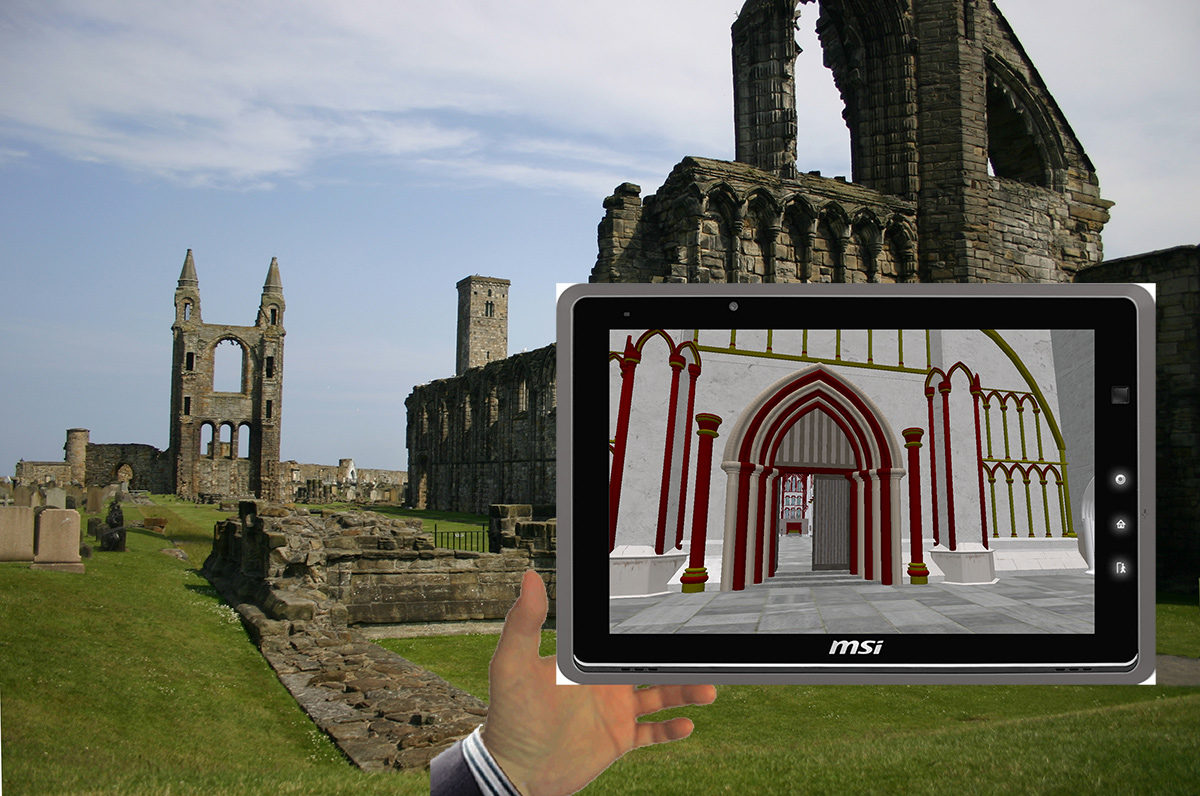
\includegraphics[width=0.49\textwidth]{mockup.jpg}
\caption{Illustration of VTW concept; simultaneously exploring the present day traces of the cathedral at St Andrews and its virtual reconstruction.}
\label{mockup}
\end{figure}

In contrast to previous alternate reality projects within the domain, the use of a virtual environment to host a complete reconstruction means that it can easily be made remotely accessible in a very similar manner as it is at the site itself. This presents many intriguing opportunities; interaction between on-site and off-site visitors, including the ability for domain experts to imbue their knowledge to site visitors even if they themselves are not at the site; continued interaction with the digital content, in a familiar fashion, after visitors have left the site; and increased accessibility of the digital content for persons unable to physically visit the real site for any reason.

We continue in section \ref{sec:background} by briefly describing the cross reality paradigm, its position in relation to other alternate realities and how it can be of benefit to cultural heritage. The Virtual Time Window project is introduced in section \ref{sec:vtw} with a high-level discussion of its design, before exploring the design space and the suitability of available technologies to the project in section \ref{sec:survey}. Our progress in implementing the project is discussed in section \ref{sec:implementationofvtw}.

\section{Cross Reality}
\label{sec:background}
Cross reality is the ubiquitous mixed reality situation that arises from the fusion of real-world sensor/actuator infrastructure with virtual environments, such that augmented reality and augmented virtuality manifest simultaneously and facilitate synchronous multi-directional exchange of media and control information between real and virtual environments. Sensors collect and tunnel dense real-world data into virtual environments where they are interpreted and displayed to dispersed users, whilst interaction of virtual participants simultaneously incarnates into the real world through a plenitude of diverse displays and actuators~\cite{Paradiso2009}.

The principle features that distinguish cross reality from other alternate realities that computer science has explored are;
\begin{enumerate}
	\item a shift from single- to bi-directional information flow between real and virtual environments~\cite{kim:practical}
	\item that both environments are complete unto themselves (but are enriched by their ability to mutually reflect, influence and merge into one another).~\cite{lifton:merging}
\end{enumerate}

Because a cross reality system is comprised of two environments, one augmented reality and the other augmented virtuality, it cannot be placed at a single point on Milgram's virtuality continuum~\cite{Milgram1999} but instead occupies two separate points, one to the left and the other to the right of the centre.

Cross reality expands upon existing alternate reality research in the domain of cultural heritage by increasing the level of interactivity between users, artefacts and sites, by coupling real world conditions more tightly to those pertaining to the digital content of the site and vice-versa, allowing each to influence the other to a greater degree. In particular cross reality; allows greater user interaction with digital content; allows conditions within the real world to affect digital content; allows conditions pertaining to digital content to affect the real world; increases the extent and amount of digital content; and allows easier and greater remote access to digital content.

\section{The Virtual Time Window Project}
\label{sec:vtw}
We have designed and begun implementation of a novel application of the cross reality paradigm to the exploration of cultural heritage sites in the Virtual Time Window (VTW) project, investigating the use of tablet computers to present visitors to a cultural heritage site with a `window' into a virtual reconstruction of the entire site as it was at an earlier point in time. Visitors view the site in its current state around them and in an earlier state through the window; simultaneous exploration of real and virtual environments. Figure \ref{mockup} illustrates this concept.

To maintain a natural and unhindered sense of exploration VTW does not require visitors to manually control navigation within the virtual environment. Changes in a tablet's position within the site are automatically reflected by a corresponding movement within the virtual environment, making use of a combination of location tracking technologies. The direction that a visitor faces is monitored by magnetometer (`digital compass') and the angle that their tablet is held at by accelerometer; this information is reflected by the direction and pitch of the camera within the virtual environment (see figure \ref{tiltdiagram}). The resulting style of interaction is similar to using a digital camera to take a photo; the screen on the back of the camera shows what the image will look like when the shutter is released, whilst with VTW the screen on the tablet shows what the site looked like in the past.

\begin{figure}[!t]
\centering
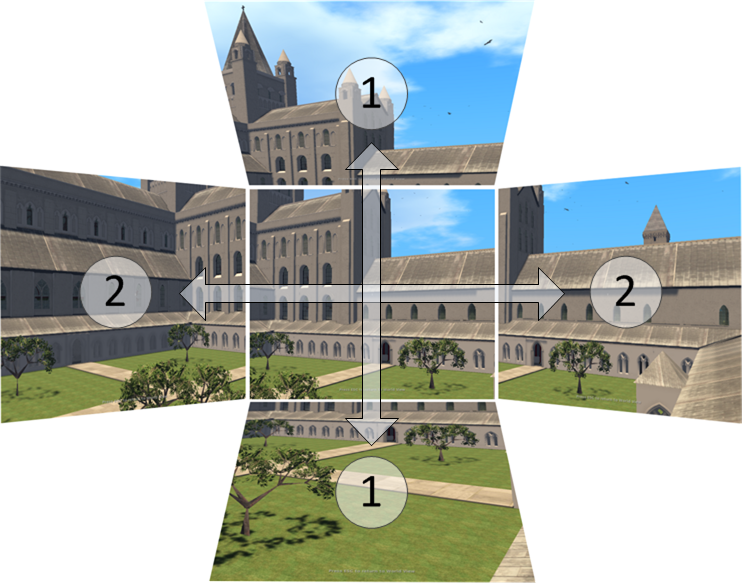
\includegraphics[width=0.49\textwidth]{tiltdiagramwarrows.png}
\caption{Illustration of how VTW maps a tablet's physical pitch (1) and bearing (2) onto virtual environment camera control.}
\label{tiltdiagram}
\end{figure}

Sensor infrastructure at the site monitors environmental and other physical properties and these data affect the state of the virtual reconstruction in real-time so that the view through the window better merges with what the user sees around it. Actuators allow interaction of visitors and scripts within the virtual reconstruction to manifest into the site, affording novel methods of explanation and demonstration of points of interest.

The design of VTW (see figure \ref{visio_diagram_2_tech}) is client-server. The server is a computer responsible for running the virtual environment server software, for distributing content to tablets running compatible virtual environment client software, and for receiving and processing sensor data (with these data affecting the content distributed to the tablets). Clients include visitors to the site itself, who are simultaneously exploring both the real site and the virtual environment with tablets, and remote visitors who are exploring only the virtual environment from elsewhere using their desktop or laptop computers. Clients also include sensors and actuators at the site, comprising both dedicated wired and wireless sensor/actuator infrastructure and mobile sensors and actuators present in the tablets.

\begin{figure}[!t]
\centering
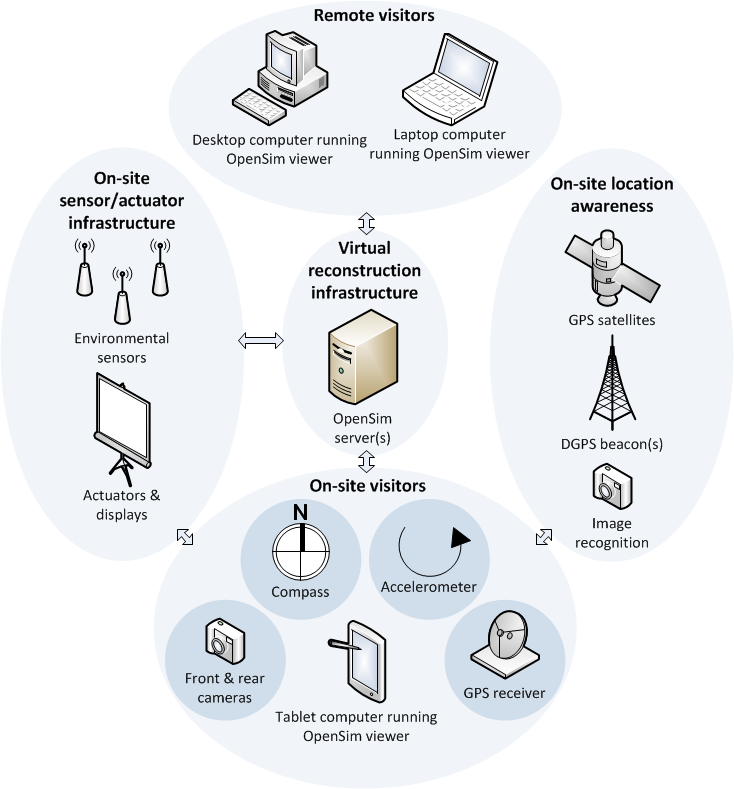
\includegraphics[width=0.46\textwidth]{visio_diagram_2_tech.png}
\caption{The main functional components and technologies of VTW from a high level of abstraction.}
\label{visio_diagram_2_tech}
\end{figure}

\section{Exploration of Design Space}
\label{sec:survey}
This section examines some of the constituent components that comprise VTW and surveys the suitability of available platforms according to the specific requirements of the project.

\subsection{Virtual Reconstruction Infrastructure}
\label{subsecvirtualreconstructioninfrastructure}
Whilst inaugural cross reality projects and the majority that have since followed have made use of virtual worlds~\cite{Sivan2009} such as Second Life~\cite{LindenResearchInc.}, OpenSimulator~\cite{OpenSimulatorProject} and Open Wonderland~\cite{OpenWonderlandFoundation}, the paradigm can also be implemented using `traditional' game and visualisation solutions such as Unity~\cite{UnityTechnologies} and Unigine~\cite{UnigineCorp}; in fact this has already occurred~\cite{mit:doppel}. However virtual worlds, particularly open virtual worlds such as OpenSim, offer researchers many benefits.

Foremost the accessibility of virtual worlds with regards to content creation makes them a more attractive option for researchers who may not have prior experience in a standalone 3D modelling package, which is a common requirement for working with game and visualisation engines. Virtual worlds provide powerful yet straightforward interfaces for building and personalising avatars, virtual spaces and objects and while these tools may lack some of the more advanced features and effects of professional modelling packages, resulting in lower photorealism, they allow researchers to create diverse and expansive environments more easily and affordably, both in terms of experience and time required~\cite{Hendaoui2008}. This allows more to be achieved within a limited budget as researchers can focus on running experiments and collecting results rather than creating the experimental environment itself.

This ability to create content and shape the virtual environment in an almost infinite number of ways, combined with the inherent open-endedness of virtual worlds and the ability to easily integrate with external data sources through application programming interfaces, streaming in video, sound and Web content, presents researchers with nearly endless possibilities, unrestricted to develop whatever styles of interaction they choose and to use the environment for whatever they wish~\cite{Warburton2009}.

These experiments can be run for extended periods of time, over a period of months or more, at very low cost, thanks to the open licensing that many virtual worlds have~\cite{Bainbridge2007}. Researchers are free to make use of existing hardware at their institution, deploy and administer their own infrastructure in any manner they see fit.

Researchers at St Andrews have used OpenSim for a number of projects, among them the accurate recreation of historical monuments including a Byzantine basilica in the Sparta region of Greece~\cite{Getchell2010} and the cathedral at St Andrews as seen in figure \ref{tiltdiagram}. We run a number of OpenSim servers and clients on a variety of different hardware, including small form factor computers that are easily transportable to public exhibition sites.

We are building upon our knowledge and experience by using OpenSim as the virtual reconstruction infrastructure component of VTW. Our physical proximity to the cathedral at St Andrews, which is a cultural heritage site of huge importance, combined with out existing OpenSim reconstruction of it, provides an ideal situation for development and testing of VTW without requiring a lengthy content creation phase.

\subsection{On-Site Sensor/Actuator Infrastructure}
\label{subsec:onsitesensoractuatorinfrastructure}
Numerous platforms for distributed sensing and actuating exist~\cite{Bose2009}. Commercially procurable hardware designed specifically for the task, such as wireless sensor network (WSN) solutions including Berkeley motes~\cite{Bose2009}, are one option whilst general-purpose low-power prototyping and embedded platforms, such as Phidgets and Arduino, have also proven popular for creation of bespoke sensor/actuator devices~\cite{Faludi2010}. Software platforms include those tailored specifically for operation on WSN motes such as TinyOS~\cite{TinyOSAlliance} and more general purpose operating systems such as Contiki~\cite{Dunkels} which is designed for running on devices with limited memory footprints and computational capabilities.

In addition to dedicated sensing infrastructure VTW uses sensors built into the tablet computers. Accelerometer and magnetometer determine tablets' orientations whilst location tracking technologies including GPS determine their position within a site. Other sensors connected to tablets can be used to detect changes in physical and environmental conditions throughout the site either to bolster data from dedicated sensing infrastructure or to allow VTW to be deployed with no dedicated sensing infrastructure; the latter scenario suits rapid deployment and withdrawal which is of particular use for temporary installations.

Actuators primarily serve as interfaces to controllable luminaires, fans, animatronics, etc. but also to more `traditional' output devices such as monitors, projectors and loudspeakers. The tablets themselves provide several output modalities; monitor, sound and vibration at a minimum.

Faced with this heterogeneity it is critical that VTW integrates with as many different sensor/actuator platforms as possible through the use of interfaces to widely adopted standards. The issue of standards is discussed further in section \ref{subsec:standards}.

\subsection{Networking}
\label{subsec:networking}
VTW relies upon networking between its constituent components; on-site clients, remote clients and server. There are several scenarios for the provision of this infrastructure, distinguished primarily by the presence or lack at the site of a suitable Internet connection and a suitable location to situate the server. Note that the server entity can comprise multiple physical computers, dependant upon the scale of the deployment.

The simplest scenario is where the site has both a suitable Internet connection and can appropriately accommodate the server physically. On-site clients communicate directly with the server via wireless networking; tablets via 802.11 and sensor/actuator infrastructure either via a low-power wireless protocol such as ZigBee (or alternatively wired Ethernet, however many sites will understandably be averse to unsightly cabling). Remote clients communicate with the server via the Internet.

If the server cannot be located on-site, for example because there is no secure and weatherproof building present, then it must be situated elsewhere, such as a datacentre, and both on-site and off-site clients must access it via the Internet. This does not change anything for off-site clients, whilst the style of communication used by on-site clients depends upon whether a suitable Internet connection is available at the site.

If this is the case then an on-site gateway communicates with the on-site clients via wireless or wired networking and marshals communications to and from the server via the Internet. This gateway is a much smaller and lower powered device than the server and can be deployed outdoors in a small weatherproof enclosure.

If a suitable Internet connection is not available then on-site clients must make use of wireless WAN connectivity such as 3G. However the default behaviour of the OpenSim client/server model is not well suited to deployment over 3G networks. Unlike online games where content such as textures and multimedia are stored on the client and communication between client and server comprise only gameplay elements such as position updates, OpenSim stores content on the server and this must be downloaded by the client each time it logs into a particular location. This is largely due to the user-generated nature of the content which means that it is susceptible to frequent change and results in high initial bandwidth requirements immediately after a client login~\cite{Bainbridge2007, Oliver2010}. However once the content has been retrieved bandwidth requirements drop substantially to levels more familiar with online games, which are theoretically attainable via 3G.

%***mention that users won't really need to alter the content, as it is a professional/accurate simulation, though then again some interesting user interaction would be nice too so maybe cache stuff but still allow users to make small additions/take copies, etc.
We are designing experiments with OpenSim and 3G networks to ascertain the feasibility of such a VTW deployment. This involves modification of an OpenSim client to allow content to be downloaded and cached whilst a suitably fast Internet connection is available, so that when a login is performed via a 3G network the only traffic that needs to be sent is movement updates and similar, with the content being read from the device's local storage. This is a realistic scenario; one can easily imagine that the tablet computers are preloaded with the necessary content before being delivered to the site where they are then loaned to visitors upon their arrival, in a similar fashion to how audio tours are already implemented at many sites.

Adoption of 4G/LTE will provide another option for on-site client communication at sites that do not have suitably fast Internet connections.

\subsection{Standards}
\label{subsec:standards}
No single standard or framework for the development of cross reality systems has been widely adopted, a situation that presents a serious challenge to the greater realisation of the paradigm through projects such as VTW.

However the advent of cross reality did not spawn the demand for standards that facilitate synchronous bidirectional flow of sensory and control information between sensor/actuator infrastructure and display technologies, whether that display is a virtual world or a traditional two-dimensional visualisation such as a graph. Sensor/actuator infrastructure was employed long before the adoption of virtual worlds as a research tool and as such there are numerous frameworks and standards that can contribute toward the creation of a cross reality system; IEEE 1451~\cite{Song2008}, Sensor Web Enablement~\cite{Botts2008}, Ubiquitous Sensor Network~\cite{kim:practical}, SenseWeb~\cite{Kansal2007}, Global Sensor Network~\cite{Aberer2006}, etc.

Previous cross reality projects have either adapted and built upon existing standards and frameworks such as these, or have developed their own bespoke and proprietary solutions. The former approach can unfortunately result in the use of standards in manners for which they were not intended nor are ideally suited for, and the latter in the creation of systems that are only compatible with particular sensor/actuator infrastructure or virtual environment platforms, which means that they cannot be easily extended by other interested parties or used as the basis for future projects.

The most promising endeavour toward alleviating this situation is ISO/IEC 23005 `Information technology - Media context and control'. Better known as MPEG-V, this is the result of 3 years work from about 30 EU-based organisations, including Philips Research, to develop a global standard for connecting different virtual worlds and for connecting virtual worlds to the real world~\cite{Gelissen2011a}.

VTW has adopted ISO/IEC 23005 not only to ensure maximum compatibility with currently available and future sensor/actuator infrastructure and virtual worlds, but also to ensure that it can be extended, built upon and integrated into future projects.

\section{Implementation of VTW}
\label{sec:implementationofvtw}
In this section we discuss our progress in implementing VTW, justifying decisions pertaining to adoption of particular hardware or software approaches to meeting certain constituent components of the designed functionality.

\subsection{Tablet Computer}
Tablet computers are used to display the OpenSim reconstruction and other associated digital content to visitors using virtual world `viewer' software. Currently such software is only available for x86/x86\_64 platforms, which limits which tablet computers can be used for the project. Currently we are using a MSI Windpad 110W 10'' tablet computer that sports an AMD Fusion Z-Series APU (dual core x86\_64 processor with Radeon HD6250 graphics)~\cite{Micro-StarInt'lCo.}.

Although popular tablet computers running Apple's iOS and Google's Android operating systems are now available with sufficiently powerful processors and graphics chipsets to produce the 3D graphics that viewers require, they are unfortunately ARM platforms which cannot run viewer software written for x86/x86\_64 platforms. We are developing VTW under the assumption that with the continued adoption of virtual worlds and the ever growing popularity of tablet computers, which are increasing in computational power and decreasing in cost with every new release, viewers written for ARM platforms will be released before the project's completion. This will greatly increase the range of supported hardware upon which VTW can be deployed.

Additional hardware considerations when determining a tablet computer's suitability for VTW is the presence of and/or compatibility with sensor and actuator devices. Most tablet computers have at least GPS, front and rear facing cameras, a tilt sensor and a light sensor built in. With an x86\_64 tablet like the Winpad, which sports a standard USB port, the connection and configuration of further devices is a trivial affair.

\subsection{Translating Tablet Location into OpenSim}
We have developed an OpenSim region module that translates a real world position specified by a latitude and a longitude into an equivalent position within an OpenSim simulation. The only requirement for this translation is the prior knowledge of a single `anchor' point within the simulation for which the equivalent latitude and longitude is known. If the simulation spans multiple adjacent OpenSim regions (squares of land 256x256 metres) then only a single anchor in one of these regions is needed for the entire simulation.

The translation is achieved by calculating the distance between the anchor's latitude and longitude and the newly supplied latitude and longitude through spherical trigonometry, specifically the haversine function which gives great-circle distance between 2 points on the surface of a sphere. This distance is then scaled according to the scale of the simulation and returned as an OpenSim vector from the anchor's position in the simulation. This allows OpenSim avatars to be moved according to readings from a GPS receiver and conceivably has many additional applications.

For the purposes of VTW, that is moving avatars within an OpenSim reconstruction of a real world cultural heritage site. the accuracy attainable from GPS even in best case scenarios is not sufficient for satisfactory user experience. Thus we are investigating the suitability of additional technologies to use in conjunction with GPS in order to attain the accuracy that we require.

Options include increasing the accuracy of GPS readings through use of a DGPS base station, or supplementing GPS readings with other location determining technologies such as image recognition, range imaging via stereo cameras, time-of-flight via radio pulses, laser rangefinding, etc.

\subsection{Translating Tablet Bearing and Orientation into OpenSim}
We have successfully used an ADXL335 3-axis $\pm$3g accelerometer connected to an Arduino to control the pitch of the camera in an OpenSim viewer. We had originally planned to use the Windpad's own tilt sensor however were unable to gain sufficient access to it, either in Windows or Linux, to use it for our purposes or even to determine its capabilities. Arduino was chosen as a convenient prototyping platform that would allow us to easily and rapidly evaluate different sensor and actuator devices, including accelerometers.

Translating readings from the accelerometer into OpenSim camera commands was achieved by programming the Arduino to mimic a standard USB joystick, with the readings from the Y axis of the accelerometer smoothed and scaled onto the Y axis of the joystick. This involved replacing the firmware on the Arduino's ATmega16u2 microcontroller, which is normally used as a USB to serial bridge for compatibility with modern personal computers that do not have serial connectors, with alternative firmware that changes the device's behaviour to that of a USB Human Interface Device (HID) with a joystick HID report descriptor~\cite{Camera}.

The major benefit of this approach is that we can use any OpenSim viewer in an unmodified form, as they all feature support for both avatar movement and camera control via USB joystick. However the viewers' `flycam' functionality that we are using to directly map the pitch of the accelerometer to the camera's pitch is not ideal for our purposes; the rest position of the flycam changes as the pitch is moved up and down, such that after a small number of pitch updates the flycam no longer returns to horizontal when the accelerometer is returned to horizontal and the calibration between the two systems is lost. There is unfortunately very little documentation available for the flycam and as such we are resorting to modifying a viewer to suit the needs of our project.

It may be possible to effect small alterations to the flycam source code in order to make it behave in the manner that we require. However as the main benefit to using the joystick and flycam approach, that it works with an unmodified client, is lost as soon as we resort to modifying a client, we are instead reverting to accessing the data from the Arduino via its normal USB to serial bridge and hooking directly into the viewer's camera control methods at a lower level, giving us much greater control and removing the dependency upon the joystick and flycam interface.

We have also begun evaluation of a HMC5883L magnetometer which, in combination with the ADXL335, allows us to determine the bearing (direction) that a tablet is facing and thus which direction the viewer's camera should be facing. The magnetometer must be used in combination with the accelerometer, as otherwise the readings are only correct when the magnetometer is held flat. As the tablet is not going to be held level, the readings from the magnetometer must be compensated using the readings from the accelerometer to gain sufficiently accurate results.

% An example of a floating figure using the graphicx package.
% Note that \label must occur AFTER (or within) \caption.
% For figures, \caption should occur after the \includegraphics.
% Note that IEEEtran v1.7 and later has special internal code that
% is designed to preserve the operation of \label within \caption
% even when the captionsoff option is in effect. However, because
% of issues like this, it may be the safest practice to put all your
% \label just after \caption rather than within \caption{}.
%
% Reminder: the "draftcls" or "draftclsnofoot", not "draft", class
% option should be used if it is desired that the figures are to be
% displayed while in draft mode.
%
%\begin{figure}[!t]
%\centering
%\includegraphics[width=2.5in]{myfigure}
% where an .eps filename suffix will be assumed under latex, 
% and a .pdf suffix will be assumed for pdflatex; or what has been declared
% via \DeclareGraphicsExtensions.
%\caption{Simulation Results}
%\label{fig_sim}eg h
%\end{figure}

% Note that IEEE typically puts floats only at the top, even when this
% results in a large percentage of a column being occupied by floats.


% An example of a double column floating figure using two subfigures.
% (The subfig.sty package must be loaded for this to work.)
% The subfigure \label commands are set within each subfloat command, the
% \label for the overall figure must come after \caption.
% \hfil must be used as a separator to get equal spacing.
% The subfigure.sty package works much the same way, except \subfigure is
% used instead of \subfloat.
%
%\begin{figure*}[!t]
%\centerline{\subfloat[Case I]\includegraphics[width=2.5in]{subfigcase1}%
%\label{fig_first_case}}
%\hfil
%\subfloat[Case II]{\includegraphics[width=2.5in]{subfigcase2}%
%\label{fig_second_case}}}
%\caption{Simulation results}
%\label{fig_sim}
%\end{figure*}
%
% Note that often IEEE papers with subfigures do not employ subfigure
% captions (using the optional argument to \subfloat), but instead will
% reference/describe all of them (a), (b), etc., within the main caption.


% An example of a floating table. Note that, for IEEE style tables, the 
% \caption command should come BEFORE the table. Table text will default to
% \footnotesize as IEEE normally uses this smaller font for tables.
% The \label must come after \caption as always.
%
%\begin{table}[!t]
%% increase table row spacing, adjust to taste
%\renewcommand{\arraystretch}{1.3}
% if using array.sty, it might be a good idea to tweak the value of
% \extrarowheight as needed to properly center the text within the cells
%\caption{An Example of a Table}
%\label{table_example}
%\centering
%% Some packages, such as MDW tools, offer better commands for making tables
%% than the plain LaTeX2e tabular which is used here.
%\begin{tabular}{|c||c|}
%\hline
%One & Two\\
%\hline
%Three & Four\\
%\hline
%\end{tabular}
%\end{table}

% Note that IEEE does not put floats in the very first column - or typically
% anywhere on the first page for that matter. Also, in-text middle ("here")
% positioning is not used. Most IEEE journals/conferences use top floats
% exclusively. Note that, LaTeX2e, unlike IEEE journals/conferences, places
% footnotes above bottom floats. This can be corrected via the \fnbelowfloat
% command of the stfloats package.

\section{Conclusion}
We have provided a brief introduction to the cross reality paradigm, a situation that arises when augmented reality and augmented virtuality take place in unison; sensor readings from a real world location trigger effects in a virtual environment whilst actions within this virtual environment simultaneously manifest into the real location via displays and actuators.

We have presented the ongoing Virtual Time Window project that applies cross reality to the domain of cultural heritage, affording simultaneous exploration of a real cultural heritage site and its virtually recreated counterpart using a tablet computer in combination with sensor/actuator infrastructure and the OpenSim virtual world platform. We believe that VTW exemplifies the worth of the cross reality paradigm outside the research lab and the importance of adopting global standards for communication between virtual worlds and between virtual worlds and the real world.

% trigger a \newpage just before the given reference
% number - used to balance the columns on the last page
% adjust value as needed - may need to be readjusted if
% the document is modified later
%\IEEEtriggeratref{15}
% The "triggered" command can be changed if desired:
%\IEEEtriggercmd{\enlargethispage{-5in}}

% references section

% can use a bibliography generated by BibTeX as a .bbl file
% BibTeX documentation can be easily obtained at:
% http://www.ctan.org/tex-archive/biblio/bibtex/contrib/doc/
% The IEEEtran BibTeX style support page is at:
% http://www.michaelshell.org/tex/ieeetran/bibtex/
\bibliographystyle{IEEEtran}
% argument is your BibTeX string definitions and bibliography database(s)
\bibliography{IEEEabrv,./bib.bib}
%
% <OR> manually copy in the resultant .bbl file
% set second argument of \begin to the number of references
% (used to reserve space for the reference number labels box)
%\begin{thebibliography}{1}

%\bibitem{IEEEhowto:kopka}
%H.~Kopka and P.~W. Daly, \emph{A Guide to \LaTeX}, 3rd~ed.\hskip 1em plus
%  0.5em minus 0.4em\relax Harlow, England: Addison-Wesley, 1999.

%\end{thebibliography}




% that's all folks
\end{document}


